\documentclass[11pt, oneside]{article}   	% use "amsart" instead of "article" for AMSLaTeX format
\usepackage{geometry}                		% See geometry.pdf to learn the layout options. There are lots.
\geometry{letterpaper}                   		% ... or a4paper or a5paper or ... 
%\geometry{landscape}                		% Activate for for rotated page geometry
%\usepackage[parfill]{parskip}    		% Activate to begin paragraphs with an empty line rather than an indent
\usepackage{graphicx}				% Use pdf, png, jpg, or eps� with pdflatex; use eps in DVI mode
								% TeX will automatically convert eps --> pdf in pdflatex		
\usepackage{amssymb}
\usepackage{amsmath}
\usepackage{parskip}
\usepackage{color}
\usepackage{hyperref}

\title{The Rocket Equation}
%\author{The Author}
%\section{}
%\subsection*{}
\date{}							% Activate to display a given date or no date

\graphicspath{{/Users/telliott_admin/Dropbox/Tex/png/}}
% \begin{center} 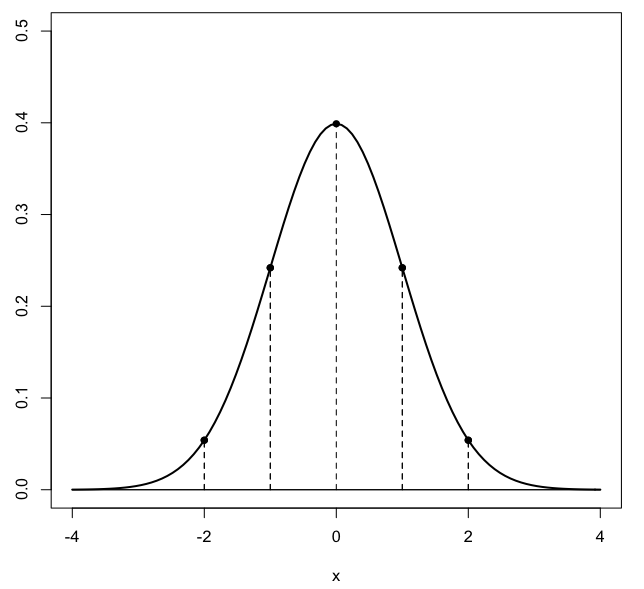
\includegraphics [scale=0.4] {gauss3.png} \end{center}
\begin{document}
\maketitle
\Large
Suppose we have a large rocket of mass $m$ which accelerates by firing hot gas out to the rear with exhaust velocity $v_e$.  The mass that is ejected is $dm$.  The initial velocity of the rocket is $v_i$ and the final velocity is $v_i + dv = v_f$.

Conservation of momentum gives us this equation
\[ mv = (m - dm)(v + dv) + (dm) (v - v_e) \]
\[ mv = mv + m \ dv - dm \ v - dm \ dv + dm \ v - dm \ v_e \]
\[ 0 = m \ dv - dm \ v - dm \ dv + dm \ v - dm \ v_e \]
\[ 0 = m \ dv - dm \ dv  - dm \ v_e \]
Ignore the term with two differentials
\[ m \ dv = dm \ v_e \]
\[ dv = v_e \frac{dm}{m} \]
\[ \Delta v = v_e \ln \frac{m}{m_0} \]

There is a sign problem here.  $m < m_0$ ??

\end{document}  